\documentclass[acmtog]{acmart}
\usepackage{graphicx}
\usepackage{subfigure}
\usepackage{natbib}
\usepackage{listings}
\usepackage{bm}
\usepackage{amsmath}

\definecolor{blve}{rgb}{0.3372549 , 0.61176471, 0.83921569}
\definecolor{gr33n}{rgb}{0.29019608, 0.7372549, 0.64705882}
\makeatletter
\lst@InstallKeywords k{class}{classstyle}\slshape{classstyle}{}ld
\makeatother
\lstset{language=C++,
	basicstyle=\ttfamily,
	keywordstyle=\color{blve}\ttfamily,
	stringstyle=\color{red}\ttfamily,
	commentstyle=\color{magenta}\ttfamily,
	morecomment=[l][\color{magenta}]{\#},
	classstyle = \bfseries\color{gr33n}, 
	tabsize=2,
	breaklines=true
}
\lstset{basicstyle=\ttfamily}

% Title portion
\title{Assignment 5:\\ {Animation with Cloth Simulation}} 

\author{Name:\quad Hidden  \\ student number:\ Hidden
\\email:\quad Hidden@shanghaitech.edu.cn}

% Document starts
\begin{document}
\maketitle

\vspace*{2 ex}

\section{Introduction}

In this project, a physically-based animation of cloth simulation is implemented. The following tasks are done.

\begin{itemize}
\item Force computation with Hooke's law
\item Structural, shear, and bending springs
\item Wind simulation
\item Obstacle collision handling
\item Drag a mesh point to move the cloth with mouse in real-time
\end{itemize}
\section{Implementation Details}

To simulate cloth movement, we divide a cloth into a number of masses, each have its own weight. The masses are connected together by virtual `springs', and can have a force on each other. 

\subsection{Transformation between world and local coordinate}

To transform a vector from local coordinate to world coordinate, we need to multiply position by the model matrix.

To transform a vector from world coordinate to local coordinate, we need to compute the inverse of the model matrix, and multiply position by it.

\subsection{Force computation using Hooke's Law}

We can compute the force between masses by Hooke's law, $F=kx$. 

The force is given by \[
	F = kx = k\cdot 
	\left(L_0 - \left\| p-q \right\|\right) \cdot 
	\frac{p-q}{\left\| p-q \right\|}
\]

where $k$ is a fixed number, $p$ and $q$ are two masses, $L_0$ is the zero-force length (distance less than this length will not cause force), and $\frac{p-q}{\left\| p-q \right\|}$ is the normalized direction of the force.

\subsection{Structural, Shear and bending springs}

Now we know how to compute forces between two masses, but we haven't implemented how masses are connected and how they can have effect on each other. We need to implement the springs.

There are three types of springs, namely \textbf{structural}, \textbf{shear} and \textbf{bend}.

\begin{itemize}
	\item \textbf{Structural springs} connect two masses that are adjacent to each other.
	
	For example, mass at position $[i,j]$ is connected to mass at position $[i+1,j], [i-1, j], [i, j+1], [i,j-1]$.

	\item \textbf{Shear springs} connect two masses that are diagonal to each other.
	
	For example, mass at position $[i,j]$ is connected to mass at position $[i+1,j+1], [i-1, j+1], [i+1, j-1], [i-1,j-1]$.
	\item \textbf{Bending springs} connect two masses that are two steps away from each other.
	
	For example, mass at position $[i,j]$ is connected to mass at position $[i+2,j], [i-2, j], [i, j+2], [i,j-2]$.
\end{itemize}

An intuitive description of the springs is shown in the following figure.

\begin{figure}[htbp]
	\centering
	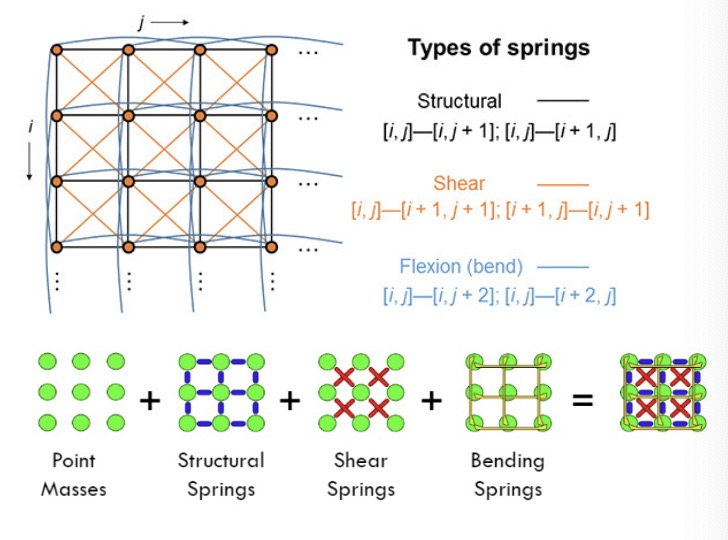
\includegraphics[width=0.4\textwidth]{images/spring-force.jpg}
	\caption{Structural, shear and bending springs}
\end{figure}

\subsection{Wind simulation}

To simulate wind, we need to apply an additional external force to the masses. Randomness is added to the wind force to make it more realistic. The cloth will be blown continously by the wind in the direction of the wind force, instead of converging to a fixed surface position.

The pseudocode is given below.

\begin{lstlisting}[language=C++, caption=Wind simulation]
void computeAcceleration(){
	// randomly generate wind force
	Vec3 wind = {0, 0, random_number / 50};

	// compute acceleration for each mass
	for (int i = 0; i < massCount; i++) {
		if (mass is pinned) continue;
		// compute force
		// ...
		// compute acceleration
		acceleration[i] = force[i] / weight;
		// add wind force
		acceleration[i] += wind / mass[i];
	}
}
\end{lstlisting}

\subsection{Sphere (obstacle) collision handling}

To simulate the collision between the cloth and a sphere, we need to compute the distance between the sphere and the cloth. If the distance is less than the radius of the sphere, we need to remove the acceleration and velocity of the masses along the direction of the normal of the sphere. Here the normal of the sphere is given by the vector from the center of the sphere to the mass.

The pseudocode is given below.

\begin{lstlisting}[language=C++, caption=Sphere collision handling]
vec3 distance = mass_pos - sphere_center;
if (length(distance) <= sphere_radius) {
	vec3 normal = normalize(distance);
	// update position
	mass_pos = sphere_center + normal * sphere_radius;
	// add 'velocity along normal' 
	// to remove velocity along sphere center
	world_velocities[i] += glm::dot(-world_velocities[i], normal) * normal;  
}
\end{lstlisting}

\subsection{Drag a mesh point to move the cloth with mouse in real-time}

To handle mouse drag event, we need to do the following steps.

\begin{enumerate}
	\item When a mouse left click is detected, we need to find out which mass the mouse is pointing at. 
	
	We accomplish this by getting the mouse position, and transform it from the screen coordinate to the world space using \verb|glm::unProject| function. The function takes in 4 arguments: the mouse position, the camera LookAt matrix, the camera projection matrix, and the viewport. The viewport is a 4-element array, which is the position of the lower-left corner of the viewport, and the width and height of the viewport. The function returns the world space position of the mouse.

	\begin{lstlisting}[language=C++]
// transform mouse position to world space
vec3 world_mouse_position = 
glm::unProject(mouse_pos, LookAtMat(), PerspectiveMat(), Vec4{0, 0, screen_width, screen_height});
	\end{lstlisting}
	
	Then we generate a ray from the camera origin to the world position we have just calculated. For each mass center, we assume it is a small sphere and do ray-sphere intersection. If the ray intersects with the sphere, we have found the mass we are looking for. We traverse each mass and find the closest one to the ray. We then set its acceleration to zero and fix its position. The pseudocode is given below.

	\begin{lstlisting}[language=C++]
// ray origin and ray direction
vec3 ray_o = camera_pos;
vec3 ray_d = glm::normalize(world_mouse_position - camera_pos);
	\end{lstlisting}

	\item When a mouse left click is maintained, it means the user is dragging the mass. We move the mass to the mouse position, and set its acceleration to zero. We also need to fix the position of the mass, so that it won't be moved by the cloth simulation.
	
	To accomplish this, similar to the previous step, we need to transform the mouse position from the screen coordinate to the world space. Then, to find out the new world position of the mass, we need to do ray-plane intersection. We assume the plane is parallel to the camera plane, and the normal of the plane is the camera direction. The plane passes through the mass. We then get the new world position of the mass. The pseudocode is given below.

	\begin{lstlisting}[language=C++]
// Plane origin and normal
vec3 normal = camera->Forward();
vec3 x0 = mass_pos[drag_index];
// Do ray-plane intersection and get 
// solution 't' of the equation
float t = (dot(normal,x0) - dot(normal,camera_pos)) / dot(normal, ray_dir);
vec3 new_pos = ray_o + t * ray_d;
	\end{lstlisting}

	\item When a mouse click is released, we simply remove the mass from the fixed mass list, so that it can be moved by the cloth simulation.
\end{enumerate}


\section{Results}

\subsection{Obstacle collision detection}

\begin{figure}[H]
	\centering
	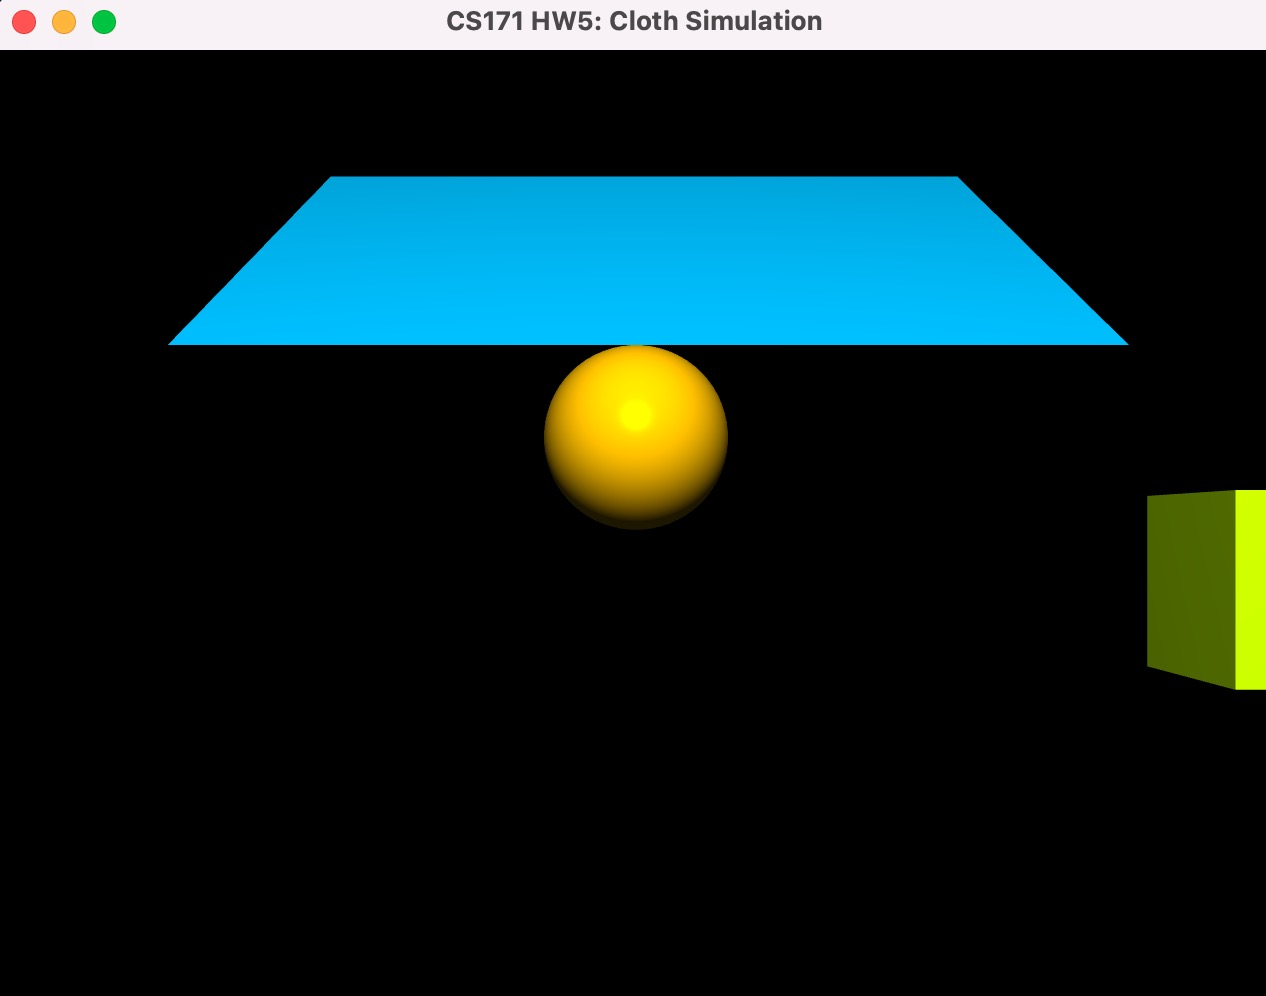
\includegraphics[width=0.4\textwidth]{results/1-initial-state.jpg}
	\caption{Initial state}
\end{figure}

\begin{figure}[H]
	\centering
	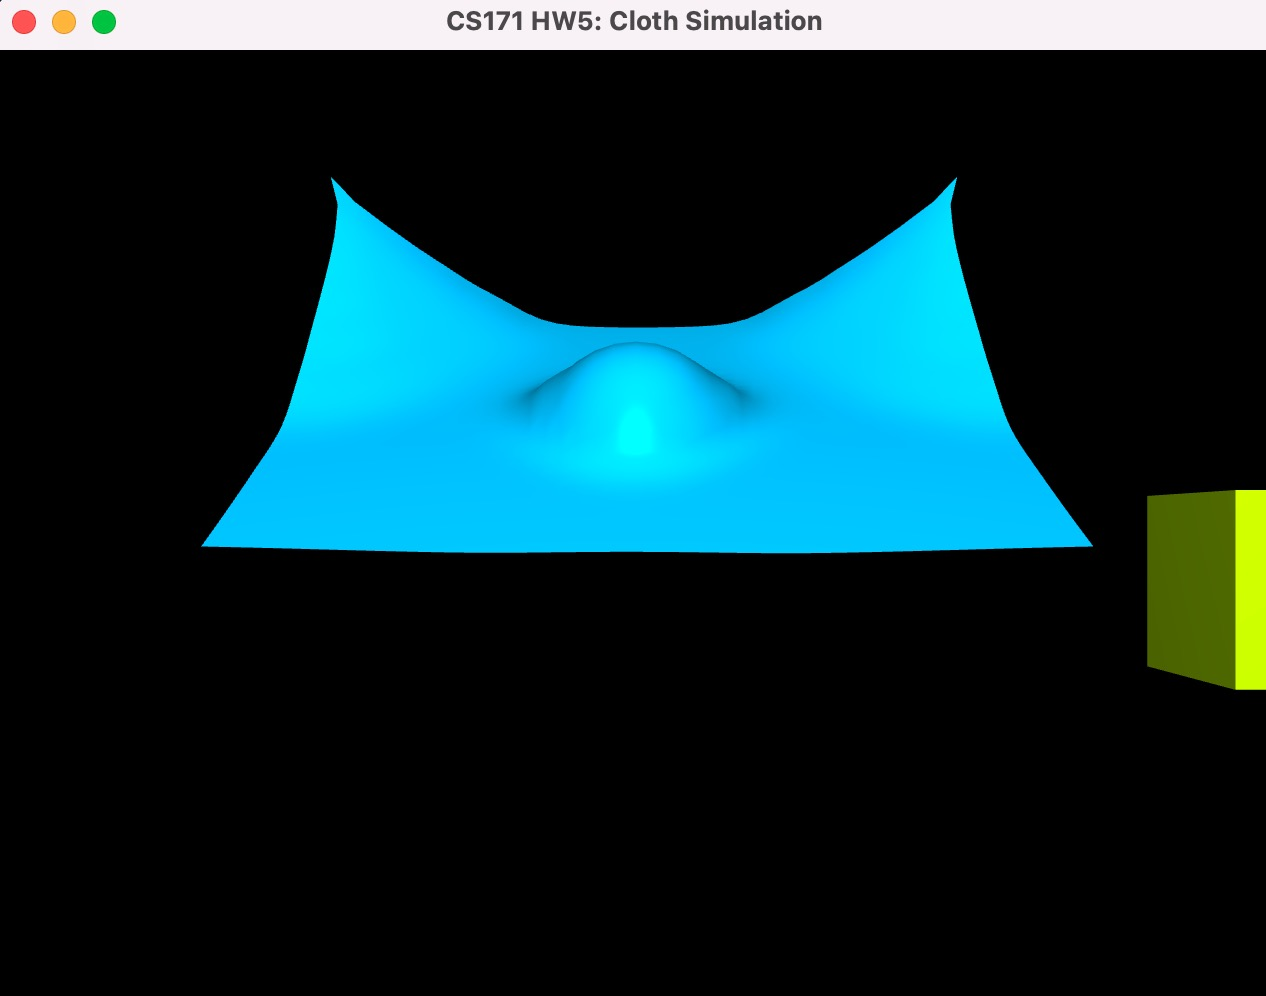
\includegraphics[width=0.4\textwidth]{results/2-falling-on-sphere.jpg}
	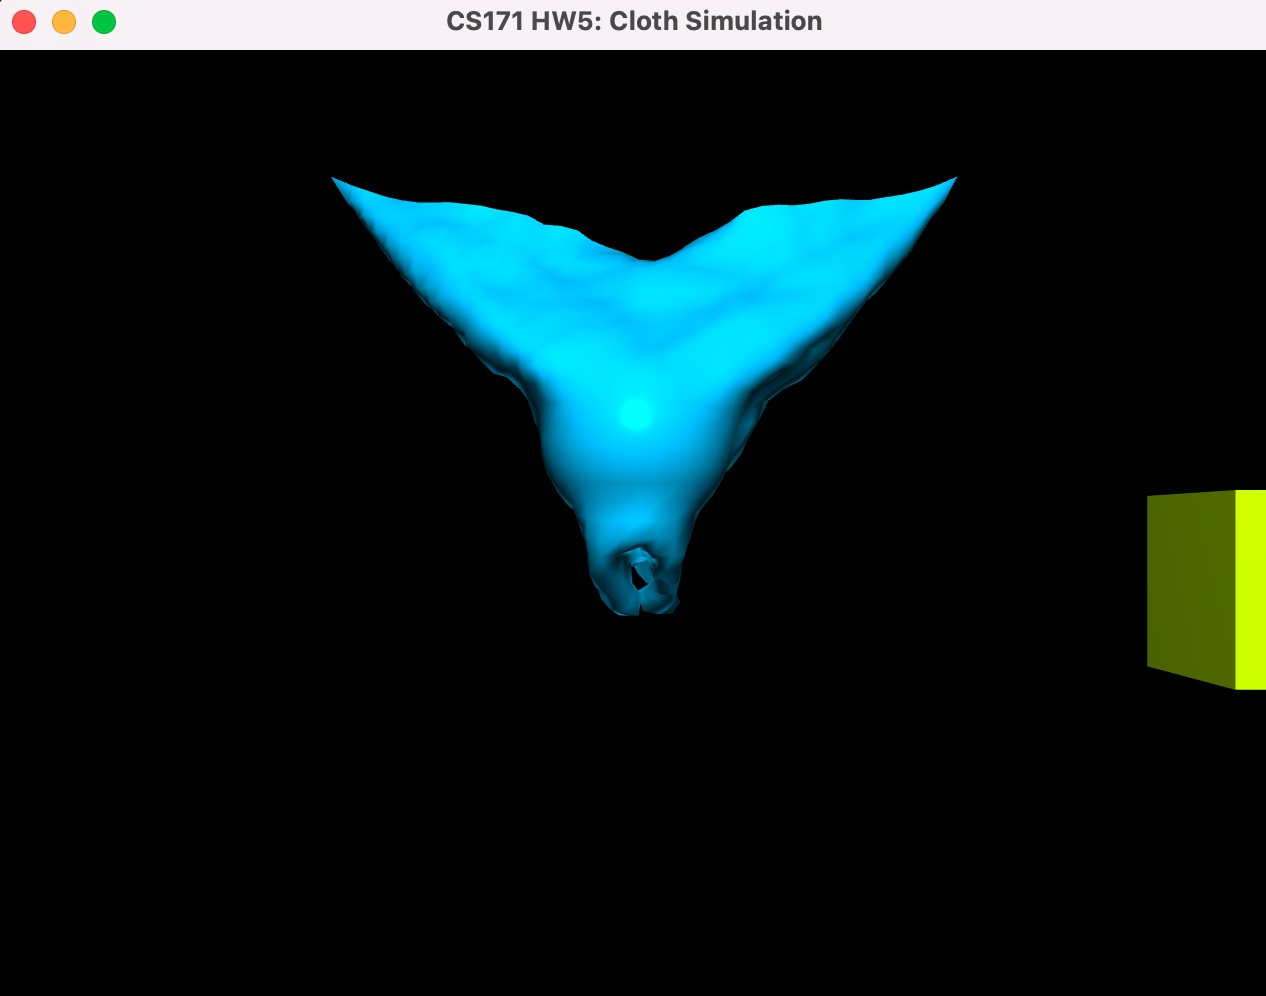
\includegraphics[width=0.4\textwidth]{results/3-falling-on-sphere-2.jpg}
	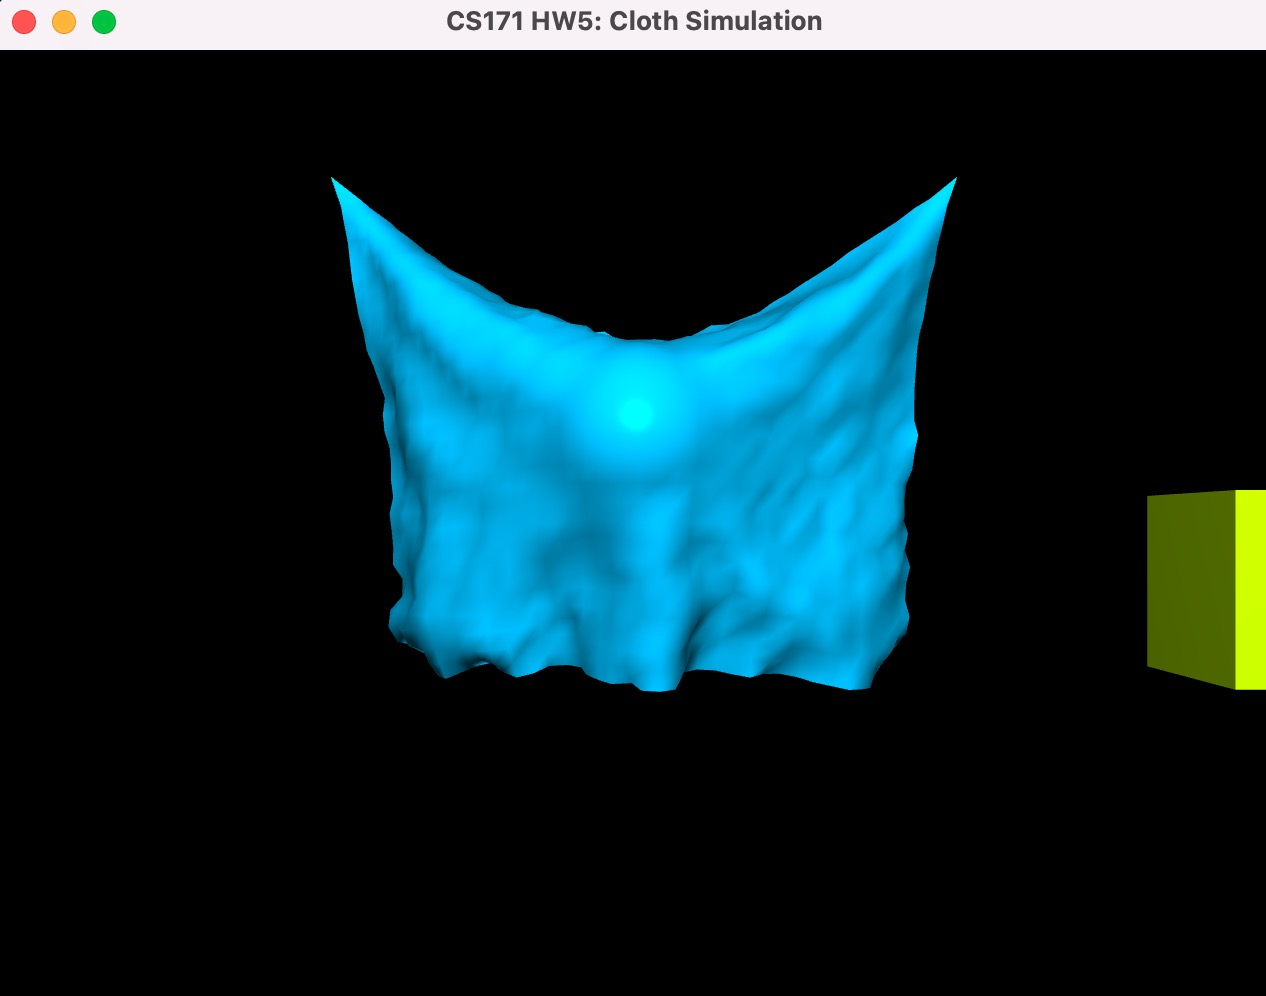
\includegraphics[width=0.4\textwidth]{results/4-falling-on-sphere3.jpg}
	\caption{Falling on a sphere}
\end{figure}

\subsection{Mouse interaction}

\begin{figure}[H]
	\centering
	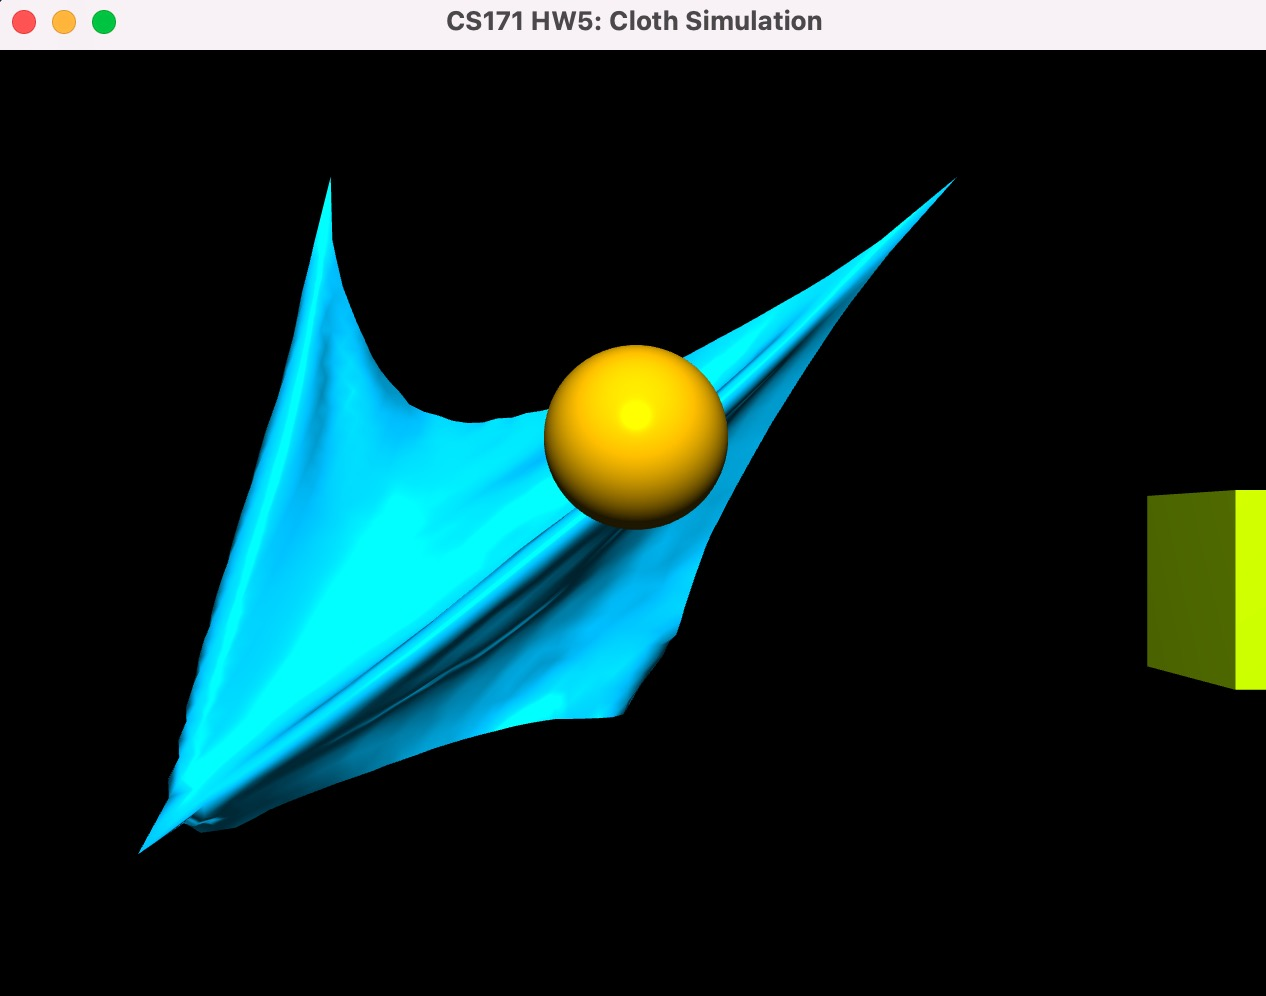
\includegraphics[width=0.4\textwidth]{results/5-mouse-drag.jpg}
	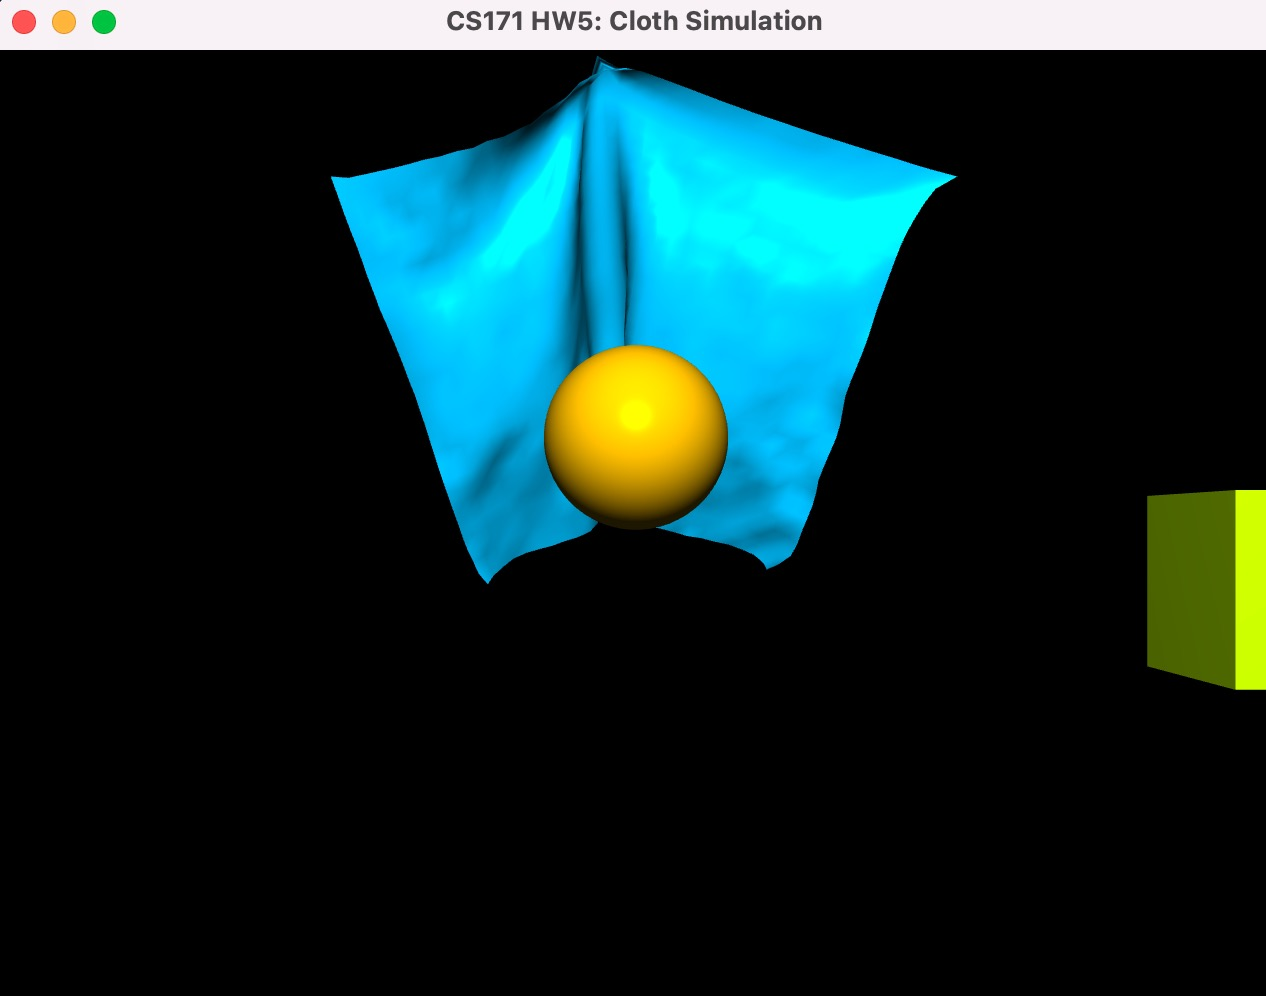
\includegraphics[width=0.4\textwidth]{results/6-mouse-drag-2.jpg}
	\caption{Drag a mesh point to move the cloth with mouse in real-time}
\end{figure}

The results will also be shown in real-time to TAs.

\end{document}
